\documentclass{beamer}
\usepackage{amsmath}
\usepackage{fourier}
\usetheme{metropolis}

% This block allows to include images and bib files relative to this TeX file.
\newcommand{\PathToTexFile}{02-presentation-v1}
\graphicspath{\PathToTexFile}

\pdfstringdefDisableCommands{%
  \def\\{}%
  \def\texttt#1{<#1>}%
}

\title{Parameter estimation\\of partial differential equations\\via neural networks}
\author{Alexander Glushko, Dmitry I.\ Kabanov}
\date{Final project on the Stochastic Numerics course\\Once upon a time in 2019}

% ------------------------------------------------------------------------------
% Useful mathematical macros
\newcommand{\Data}{\vec{D}}
\newcommand{\DataExt}{\widetilde{\vec{D}}}
\newcommand{\MSE}{\ensuremath{\text{MSE}}}
\newcommand{\T}{\ensuremath{\text{T}}}
\renewcommand{\vec}[1]{\boldsymbol{#1}}
\newcommand{\VTheta}{\ensuremath{\vec{\theta}}}
\newcommand{\VLambda}{\ensuremath{\vec{\lambda}}}
\DeclareMathOperator*{\argmin}{arg\,min}
\newcommand{\R}{\mathbb R}
\newcommand{\UNN}[1][\text{NN}]{u_{#1}}
\newcommand{\FNN}[1][\text{NN}]{f_{#1}}
\newcommand{\NonlinOp}{\mathcal N\!}
% Useful mathematical macros (end)
% ------------------------------------------------------------------------------

\begin{document}
\maketitle

% ------------------------------------------------------------------------------
% Common part
\begin{frame}{Outline}
\begin{itemize}
    \item Introduction to the problem of parameter estimation of PDEs
    \item Solution set up
    \item Description of neural networks
\end{itemize}
\end{frame}

%slide 2
\begin{frame}{Introduction to the problem}

The main goal fo our project is:

Given data $\vec{D} = \{t_i, x_i, u_i\},`~i = 1, ..., N,$ observed from the solution of PDE of the form
\begin{equation}
    \label{eq:pde}
    u_t + \mathcal N\!(u; \VLambda) = 0,
\end{equation}
estimate $\VLambda$.

Here $u=u(x, t)$ is the solution of the equation,
$\NonlinOp(u; \VLambda)$ a nonlinear algebraic-differential operator,
$\VLambda$ the vector of unknown parameters.

\end{frame}

%slide 3
\begin{frame}

By Bayes' rule, the optimal value of $\VLambda$ is found through
maximization of the posterior distribution \cite{sivia2006data}
\begin{equation}
    \rho( \VLambda | \Data ) \propto
    \rho( \Data | \VLambda ) \times \rho( \VLambda ).
\end{equation}

Furthermore, we assume
\begin{equation}
    u_i = u(x_i, t_i; \VLambda) + \epsilon_i, \quad i=1, \dots, N,
\end{equation}
where $\epsilon_i \sim N(0, \sigma^2)$, and assign uninformative prior for $\VLambda$
\begin{equation}
    \rho(\vec{\lambda}) = \text{const} \quad \text{ for all } \vec{\lambda},
\end{equation}
so that, the problem of finding $\VLambda$ is a nonlinear unconstrained
optimization problem
\begin{equation}
    \label{eq:optim-ideal}
    \argmin_{\VLambda} \quad 
    \log \sum_{i=1}^{N} \big[ u_i - u(x_i, t_i; \VLambda) \big]^2,
\end{equation}
here noise variance $\sigma^2$ is a~
nuisance parameter~\cite[section~8.2]{sivia2006data}
    
\end{frame}

% slide 4
\begin{frame}

Analytical solution of the optimization problem~\eqref{eq:optim-ideal} can be expensive, so following \cite{raissi2017pinnII}
we replace  $u(x_i, t_i; \VLambda)$ with a 
feedforward neural network \cite{goodfellow2016deep}. The description of the neural network will be presented in the slides below.

Furthermore, to ensure that $\UNN( x, t; \VTheta)$
is close to the exact solution of Eq.~\eqref{eq:pde}, we formulate the problem of estimating of the unknown parameters
$\VLambda$:
\begin{subequations}
\label{eq:optim}
\begin{align}
    &\argmin_{\VLambda, \VTheta} \quad \ \ 
        \sum_{i=1}^N \big[u_i - \UNN(x_i, t_i; \VTheta)\big]^2  \\
    &\text{subject to } \ \ \UNN[\text{NN}, t]  + \NonlinOp(\UNN; \VLambda) = 0.
\end{align}
\end{subequations}

\end{frame}

% slide 5
\begin{frame}
The equality constraint is difficult to satisfy exactly as
$u_{\text{NN}}$ is an approximation of the exact solution of
Eq.~\eqref{eq:pde}.
Therefore, we relax the optimization problem introducing a secondary NN
\begin{equation}
    \FNN(x, t; \VLambda, \VTheta) =
        u_{\text{NN}, t} + \NonlinOp(u_{\text{NN}}; \VLambda),
\end{equation}
where we plug the neural network $\UNN$ into Eq.~\eqref{eq:pde} and
require that $\FNN \approx 0$.

Then both networks are trained simultaneously:
\begin{equation}
    \argmin_{\VLambda, \VTheta}
    \sum_{i=1}^N \big[ u_i - \UNN(x_i, t_i; \VTheta)\big ]^2
    +\gamma \sum_{i=1}^N \big[ \FNN(x_i, t_i; \VLambda, \VTheta) \big]^2,
\end{equation}
where $\gamma$ is an extra hyperparameter that controls the importance of the
penalty term.
This parameter $\gamma$ is chosen via cross-validation and bayesian regularization.
    
\end{frame}

%slide 6
\begin{frame}{Description of neural networks}
    
Let us recall the neural network equation:
$$
\UNN(x, t; \vec{\theta}) = g_L \circ g_{L-1} \circ \dots \circ g_1,
$$
where
\[
    g_\ell(z; \VTheta_\ell) = \sigma (W_\ell z + b_\ell), \quad \ell = 1,\dots,L.
\]
Here 
\begin{itemize}
    \item $L$  - is the number of layers in the network,
    \item 0 layer and $L$ layer are input and output layers, respectively,
    \item layers from 1 to $L-1$ - are hidden layers,
    \item $\sigma = \tanh (z) $ - is a nonlinear activation function applied componentwise.
\end{itemize} 
 
The neural-network parameter $\VTheta$ contains the components of matrices
$W_\ell \in \R^{n_{\ell}\times n_{\ell-1}}$ and bias vectors
$b_\ell \in \R^{n_\ell}$, where $n_\ell$  (number of "neurons") denotes the width of the
$\ell$\textsuperscript{th} layer.
    
\end{frame}

% slide 7
\begin{frame}

Below, one can see the scheme of the neural network that we use in this project:
\begin{figure}
\centering
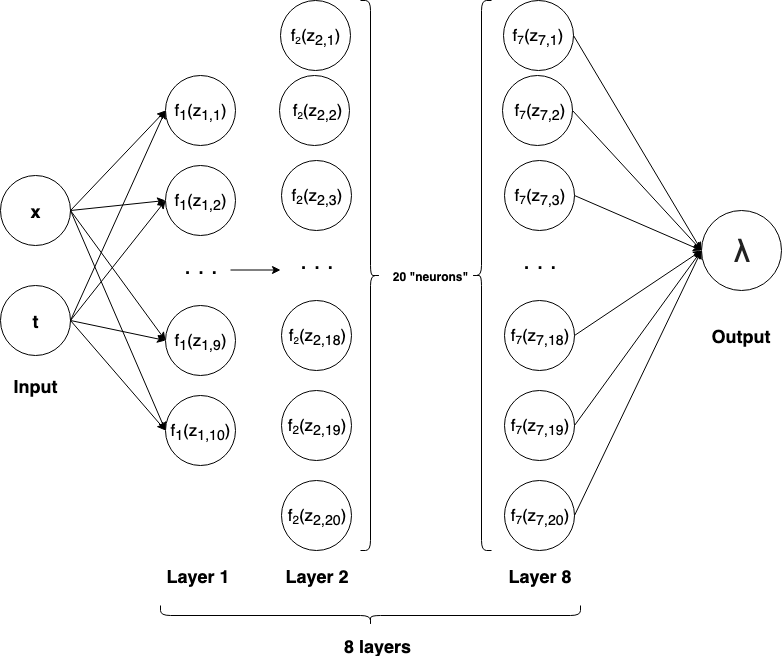
\includegraphics[width = 10cm , height = 6cm]{images/NN_scheme.png}
\\
\caption{Figure 1. Physics informed neural network.}
\end{figure}
\end{frame}

%slide 8
\begin{frame}

As one can see on the Figure 1., we use the first layer as input data driven
form the equation (1). As an activation function, we use $\sigma = tanh(z)$. We
use $tahn(z)$ as its derivative has a good behavior in the region $[-1, 1]$
\cite{nndesign}. In total, the neural network has 10 layers. 6 of them have a
width of 20 "neurons". Below, we will show the dependence of the resulting value
$\lambda$ on the neural network configuration. Especially, the affection of the
number of hidden layers in the network.
    
\end{frame}

%slide 9 
\begin{frame}

Below, one can see the table of the output $\vec{\lambda}$ values depending on
the network configuration for Burgers' equation. Here we have the relative
error: $\frac{\vert \lambda_i - \lambda_{i~True}\vert}{\lambda_{i~True}},~ i =1,
2$
\begin{table}
\begin{center}
\begin{tabular}{||c | c | c | c | c||} 
\hline
Configuration & $\lambda_1$ & Error $\lambda_1$ & $\lambda_2$ & Error $\lambda_2$ \\ 
\hline\hline
[2, 10, 1] & 0.7347 & 26.527 & 0.00537 & 68.703 \\
\hline
[2, 20, 1] & 0.7398 & 26.0326 & 0.004882 & 53.3654 \\
\hline
[2, 10, 20, 1] & 0.951 &  4.89992 & 0.0044454 & 39.65582 \\
\hline
[2, 10, 20x2, 1] & 0.9975185 & 0.248152 & 0.003245 & 1.9329 \\
\hline
[2, 10, 20x3, 1] & 0.99794 &  0.20582 & 0.0032 & 0.614 \\
\hline
[2, 10, 20x4, 1] & 1.00022 & 0.02117 & 0.00321 & 0.2508 \\
\hline
[2, 10, 20x5, 1] & 0.99963 & 0.0374 & 0.003221 & 1.1881 \\
\hline
[2, 10, 20x6, 1] & 0.99985 & 0.01495 & 0.0031793 & 0.120 \\
\hline
\end{tabular}
\caption{Table 1. Dependence of the $\vec{\lambda}$ on the number of network layers.}
\end{center}
\end{table}
    
\end{frame}

%slide 10
\begin{frame}

As one can see in Table 1., the network output directly depends on the network length. 
    
\end{frame}

% Common part (end)
% ------------------------------------------------------------------------------


% ------------------------------------------------------------------------------
% Heat equation part

\section{Example 1. Heat equation}

\begin{frame}{Heat equation}
    We consider linear heat equation with homogeneous Dirichlet boundary
    conditions
\begin{align*}
    &u_t - \lambda u_xx - g(x, t) = 0, \quad x\in[-1; 1], \quad t\in[0, 1] \\
    &u(x, 0) = 0 \\
    &u(0, x) = u(1, x) = 0
\end{align*}
with source term $g(x, t) = (4\pi^2 -1) \, \sin(2\pi x) \, \exp(-t)$.

True value of $\lambda$ is 1.
\end{frame}

\begin{frame}{Observations}
The exact solution $u = \sin(2\pi x) \, \exp(-t)$ is given on the uniform grid
with 201 points in $x$ and 101 points in $t$. 
We sample 3200 observations uniformly.

\centering
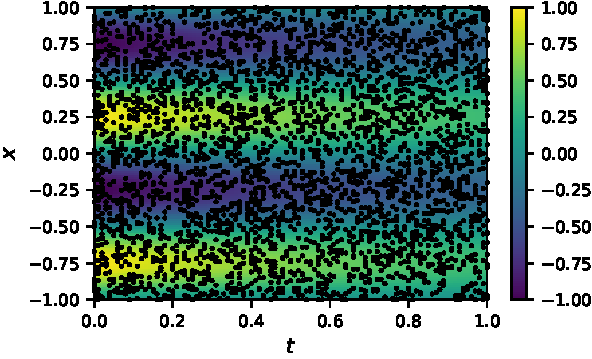
\includegraphics{images/heateq-observations}
\end{frame}

\begin{frame}{Preliminary results with $\gamma=2$}
Training the network with $\gamma=2$ gives prediction $\widehat{\lambda} =
1.00175$ with error $\approx 0.18 \,\%$.

\vspace{0.5cm}
\centering
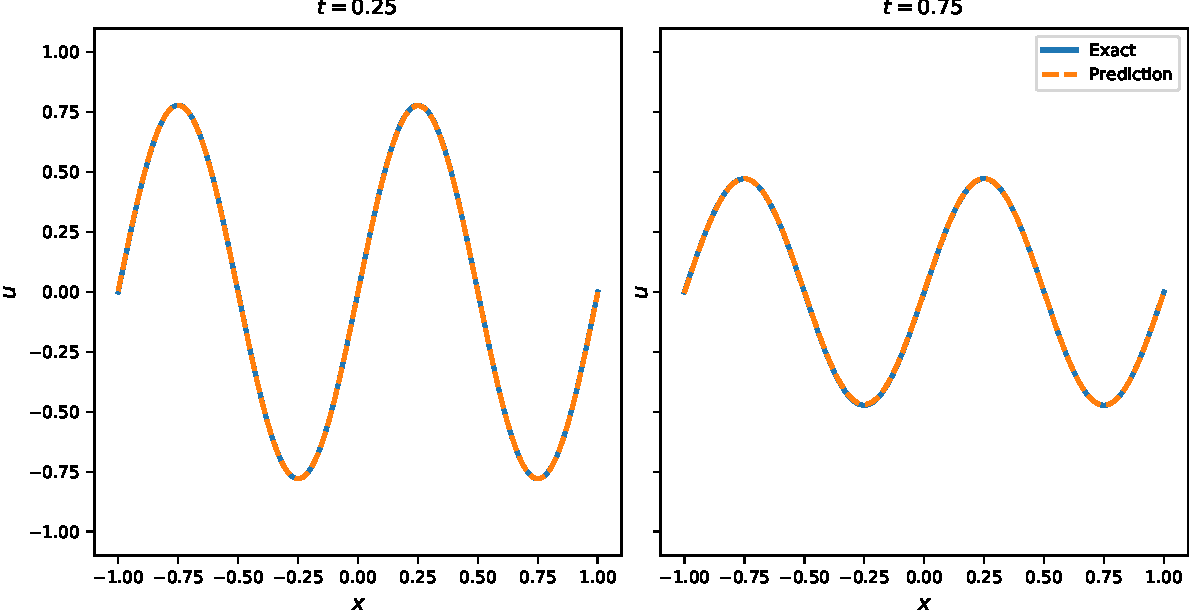
\includegraphics[scale=0.55]{images/heateq-predictions}

\end{frame}

% Heat equation part (end)
% ------------------------------------------------------------------------------


% ------------------------------------------------------------------------------
% Burgers' equation

\section{Burgers' equation}

%slide 10
\begin{frame}

Let us consider the Burgers' equation. This equation is nonlinear and serves as a prototype of the governing equations of fluid dynamics \cite{comp1986fluids}. 
\begin{equation}
    \frac{\partial u}{\partial t} + u \frac{\partial u}{\partial x} = \nu^2 \frac{\partial^2 u}{\partial x^2}
\end{equation}
For small values of the viscosity parameter $\nu$ , Burgers' equation can lead to shock formation that is notoriously hard to resolve by classical numerical methods. 

\end{frame}

% slide 11
\begin{frame}
In this project we are going to consider the input data of the following form of
the Burgers' equation:
\begin{align}
u_t + u u_x - (0.01/\pi)u_{xx} = 0, x \in [-1, 1], t \in [0, T], &\\
u(0, x) = -sin(\pi x), & \\
u(t, -1) = u(t, 1) = 0.&
\end{align}
As we are solving the inverse problem, our goal is to find values:
\[
    \lambda_1 = 1,  \lambda_2 = (0.01 / \pi) \approx 0.318
\]
using the
following input data matrices: 
\begin{align}
t \in [0, 1] \text{ of size } [100, 1], \\ x
\in [-1, 1] \text{ of size } [256, 1], u \text{ of size } [256, 100]
\end{align}

\end{frame}

% slide 12
\begin{frame}

Optimizing all loss functions using L-BFGS (a quasi-Newton, full-batch gradient-based optimization algorithm \cite{Liu1989Nocedal}), we have got the following bootstrapped results:

\begin{figure}
\centering
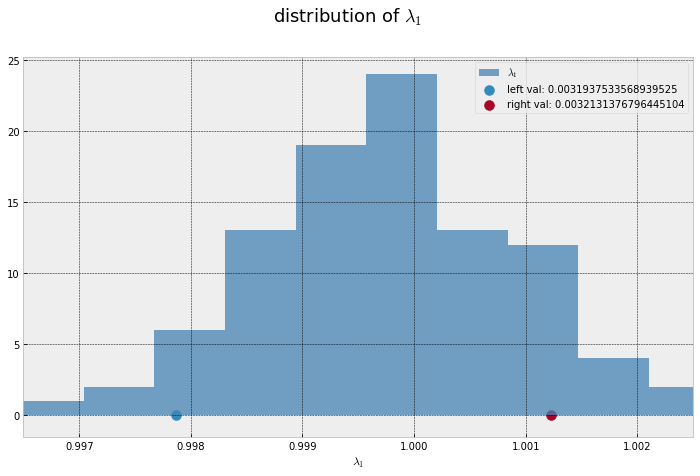
\includegraphics[width = 5.7cm , height = 4cm]{images/l1_confidence.png}
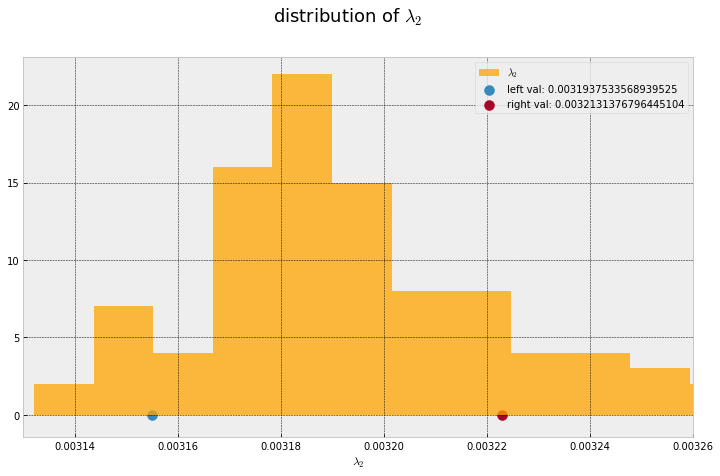
\includegraphics[width = 5.7cm , height = 4cm]{images/l2_confidence.png}
\\
\caption{Figure 1. Bootstrapped parameters $\lambda_1$ and $\lambda_2$ for Burgers' equation.}
\end{figure}

\end{frame}

% slide 13
\begin{frame}

The panel of Figure 2 shows the predicted solution u(t,x) along with the
locations of the initial and boundary training data. This prediction is obtained
without any sort of discretization of the spatiotemporal domain. 

\begin{figure}
\centering
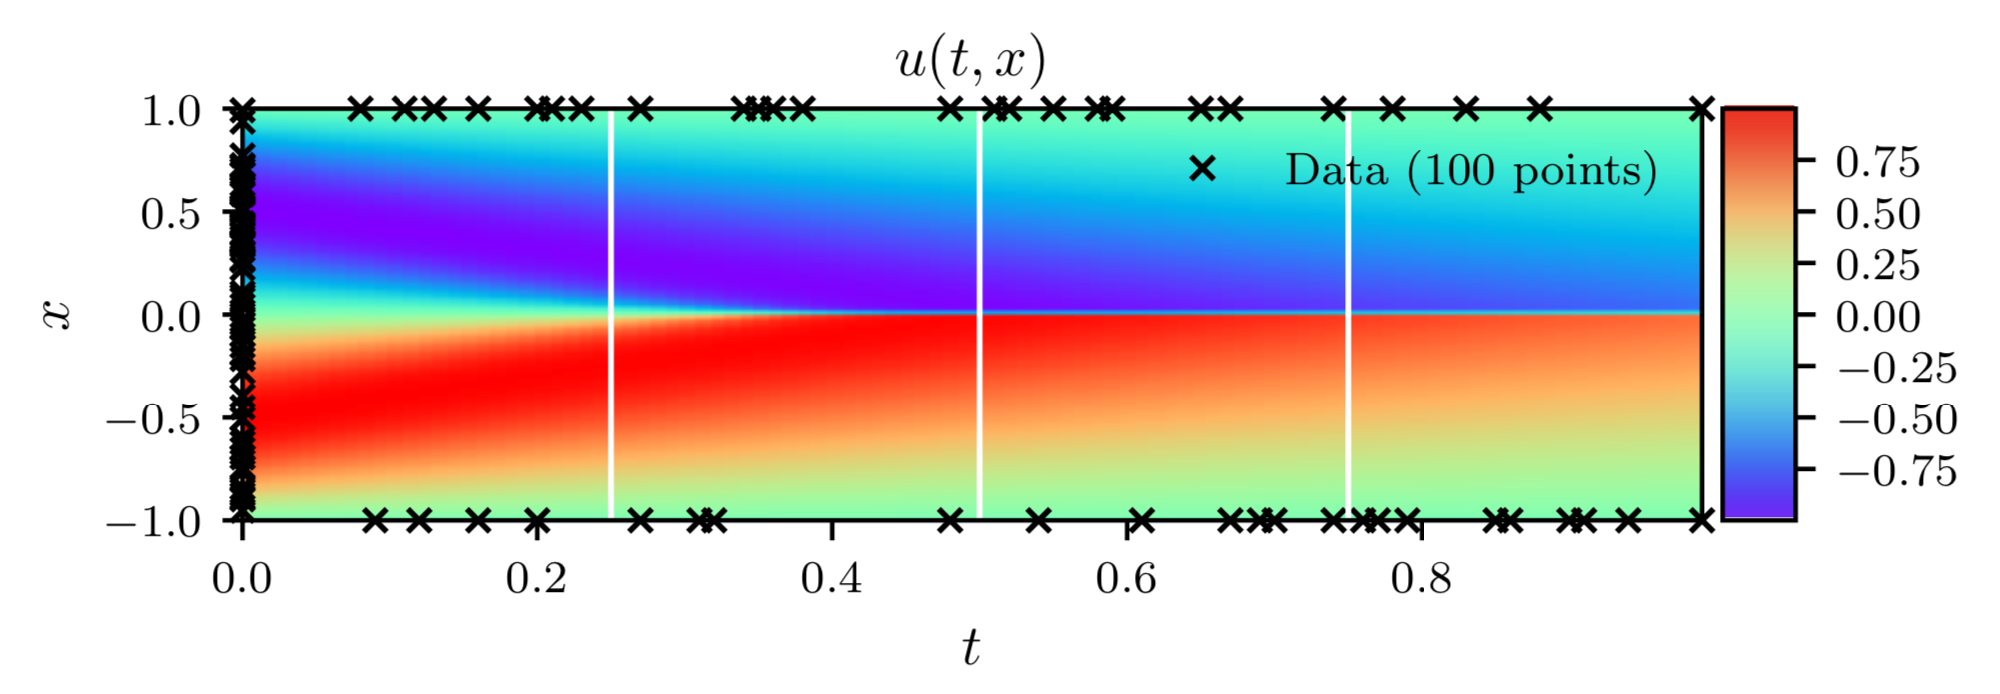
\includegraphics[width = 10cm , height = 4cm]{images/predicted_sol_burgers.png}
\\
\caption{Figure 2. Predicted solution $u(t,x)$ along with the initial and
boundary training data.}
\end{figure}

\end{frame}

% slide 14
\begin{frame}

Below, we present a comparison between the exact and the predicted solutions at
different time instants t = 0.25, 0.50, 0.75. The physics informed NN accurately
captures the nonlinear behavior of the Burgers' equation that leads to the
development of a sharp internal layer around t = 0.4.
    
\begin{figure}
\centering
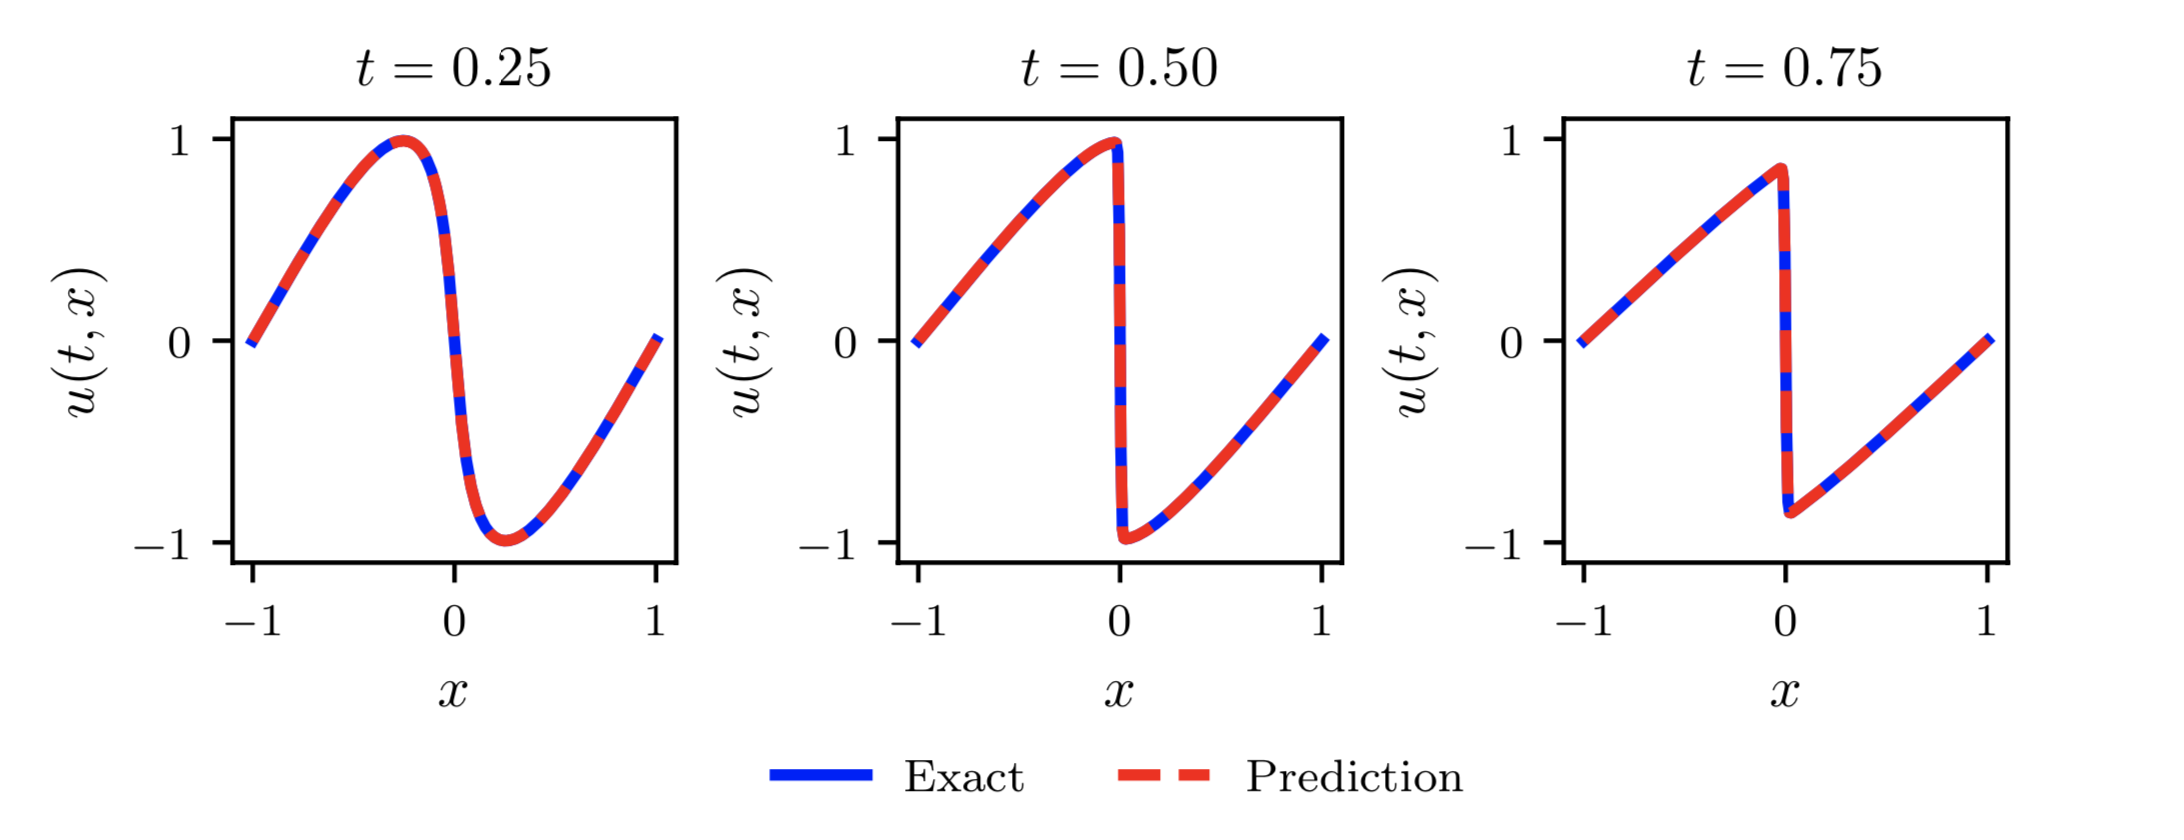
\includegraphics[width = 8cm , height = 4cm]{images/exact_pred_burgers.png}
\\
\caption{Figure 3. Comparison of the predicted and exact solutions
corresponding to the three temporal snapshots depicted by the white vertical
lines in the top panel.}
\end{figure}

\end{frame}

% slide 15
\begin{frame}

Therefore, a key property of physics informed neural networks is that they can
be effectively trained using small data sets; a setting often encountered in the
study of physical systems for which the cost of data acquisition may be
prohibitive.
    
\end{frame}

% Burgers' equation (end)
% ------------------------------------------------------------------------------

\begin{frame}
    \frametitle{Conclusions}

\end{frame}


\bibliography{presentation}
\bibliographystyle{abbrv}

\end{document}
